\section{Presentation Logic Layer}

The website will be divided into the following pages:
\begin{itemize}
    \item Landing page: The main purpose of the landing page is to encourage visitors to take action including log in or sign up for WrokFlix website.
    \item Board page: it is created under a workspace to organize tasks. On a board page, users can keep track of information about projects and workflows, which helps you collaborate with your colleagues.
    \item LogIn SignIn page: allows the users login and register to the web application. 
    \item TemplatePage page: display templates for users to use.
    \item User Setting page: allows the users to edit her or his profile information.
    \item Analytics page: allows the manager of the workspace to view the analytics data.
    \item Workspace page: allows user to manage her or his workspace.
\end{itemize}


%For the main pages put a draft and describe it in detail.
\subsection{Landing Page}
The landing page is divided into two sections: “header” and “body”. \\
In the 'Header' area, there are two sub-sections. On the left, the logo of our 
website 'WorkFlix' is displayed. In the second homework, our team will design the log.
On the right, the main navigation is composed of two major functions of the landing page, namely, log-in and sign-up.
By clicking on the text, users will be directed to the login and sign-up page.\\
In the 'Body' area, the container is divided into two parts. 
The left part is the slogan to attract users' attention and demonstrate WorkFlix's main function.
Under the slogan, there is a button for users to sign up. 
The left part is an image banner, which uses an image to highlight the website's using scenario. \\


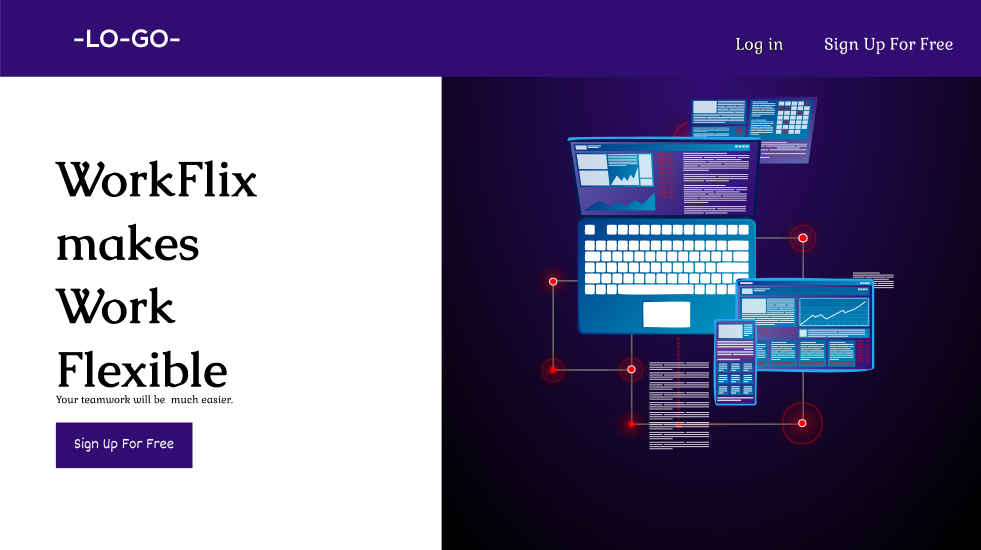
\includegraphics[width=\columnwidth]{images/LandingPage.png}
\subsection{Board Page}

A board page is a page created under a workspace to organize tasks. On a board page, users can keep track of information
about projects and workflows, which helps you collaborate with your colleagues.\\

Once users have selected a workspace, they can create different board pages in the workspace A workspace can have multiple
boards at the same time. Click on one of them to go to the board page.\\

On board page users can create lists in their boards. Lists take cards, or specific tasks, and organize them by their
various stages of progress. Lists can be used to create a workflow. By clicking "Add another list", entering the list
title and clicking Add List, you can add your new list to your board page.\\

Users can create the required tasks to the list by adding cards.Just click “Add a card…” at the bottom of any list to create
a new card, and give it a name.Cards can be customized to hold a wide variety of useful information by clicking on them. By
clicking the Edit button, you can add, delete and change the activity, for example, modify the activity label, add or delete
members associated with the activity, add or delete time associated with the activity, and also move the card from start to
finish for each step of the process.
\includegraphics[width=\columnwidth]{images/Board.jpg}








\subsection{Template Page}

A template in a web application refers to a pre-designed layout or structure that can be customized to create a new web page or website.\\

Templates typically include the basic elements of a web page, such as headers, footers, navigation menus, and content sections, which can be modified to fit the specific needs of the user.\\

Templates can be created from scratch, or they can be downloaded from a library of pre-built templates, which are often available for free or for a fee.\\

Web developers and designers use templates to save time and streamline the web development process.
\includegraphics[width=0.8\columnwidth]{images/template.jpg}

\subsection{User Setting}

User settings in a web application refer to the customizable options and preferences that users can set to personalize their experience within the application.\\

User settings may include options such as language preferences, time zone settings, font size, color schemes, notification preferences, privacy and security settings, and more.\\

These settings can enhance the user experience by allowing users to tailor the application to their specific needs and preferences.\\

User settings are typically accessed via a user profile or settings page within the web application and can be modified at any time by the user.\\

User settings can also include features like account management, password and email settings, and social media integrations.\\

By providing users with control over their experience, web applications can improve user engagement and satisfaction.\\
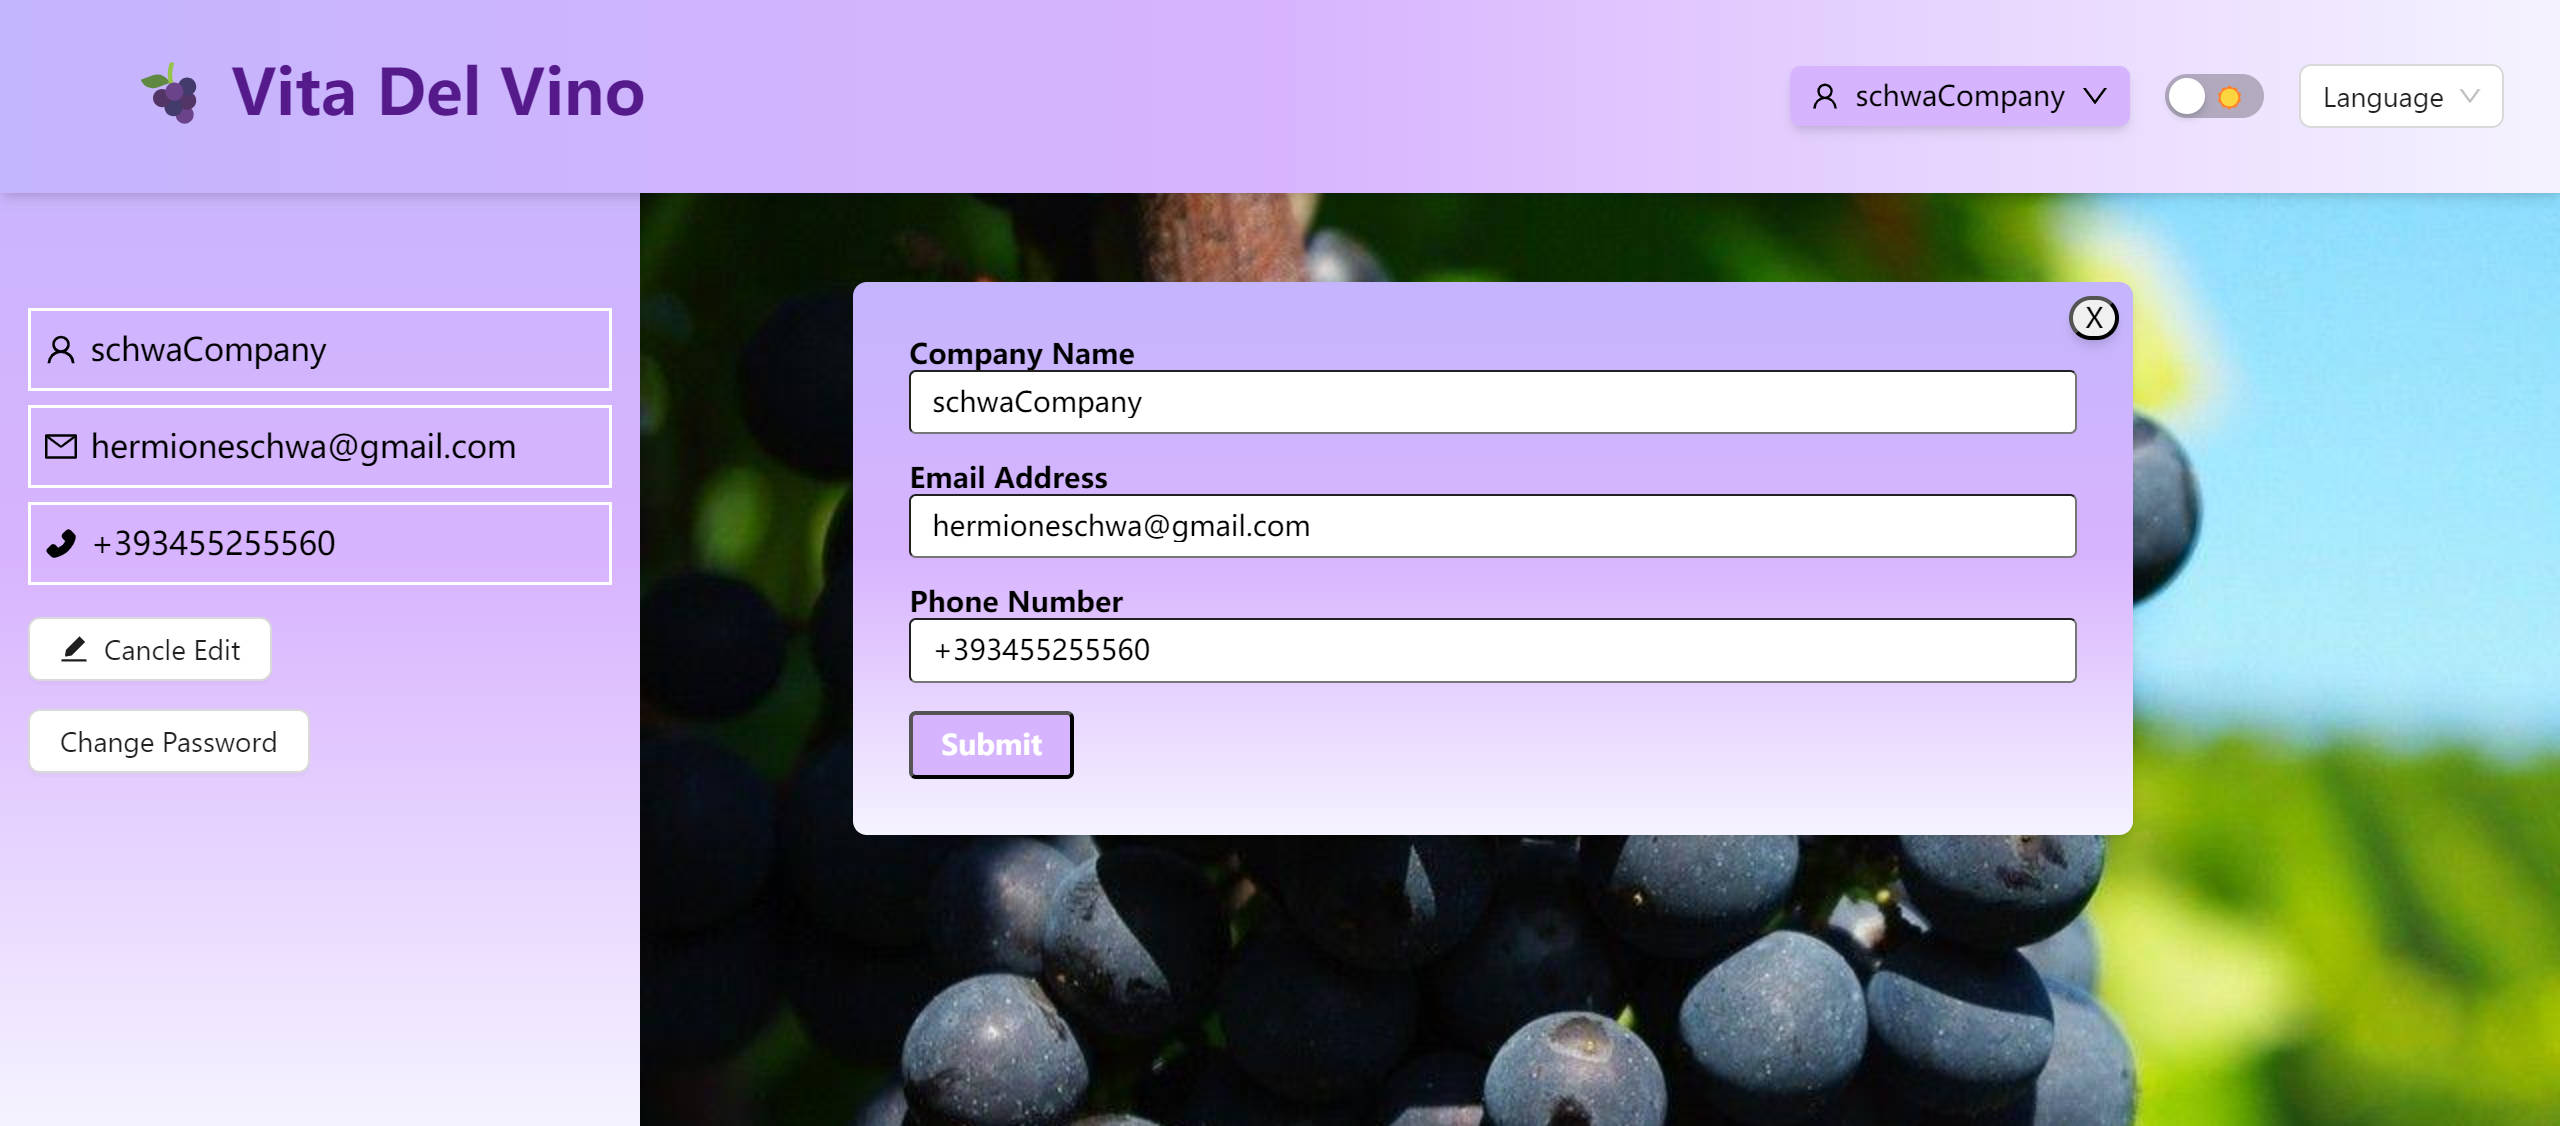
\includegraphics[width=\columnwidth]{images/UserSetting.jpg}



\subsection{Workspace}

In a web application, a workspace refers to a virtual environment where users can collaborate and work on projects, tasks, or documents together.\\

Workspaces typically include tools for communication, file sharing, project management, and other collaborative features that allow users to work together in real-time.\\

Workspaces can be used for a variety of purposes, such as team collaboration, project management, online learning, and more. Users can typically create their own workspaces or be invited to join existing ones by other users or administrators.\\

Workspaces can be accessed via a web browser or mobile application and can be customized to fit the specific needs of the users.\\
\includegraphics[width=\columnwidth]{images/Workspace.jpg}

\subsection{SignIn Login}

In a web application, "sign in" or "login" refers to the process of accessing a user's account within the application by providing the appropriate credentials, such as a username or email address and password.\\

The purpose of the sign-in process is to authenticate the user and grant access to the application's features and content that are specific to the user's account.\\

Typically, the sign-in or login page is the first page a user encounters when accessing a web application and requires the user to enter their credentials before proceeding to the main dashboard or homepage.\\

The sign-in process is essential for ensuring the security and privacy of the user's account and data within the web application.\\
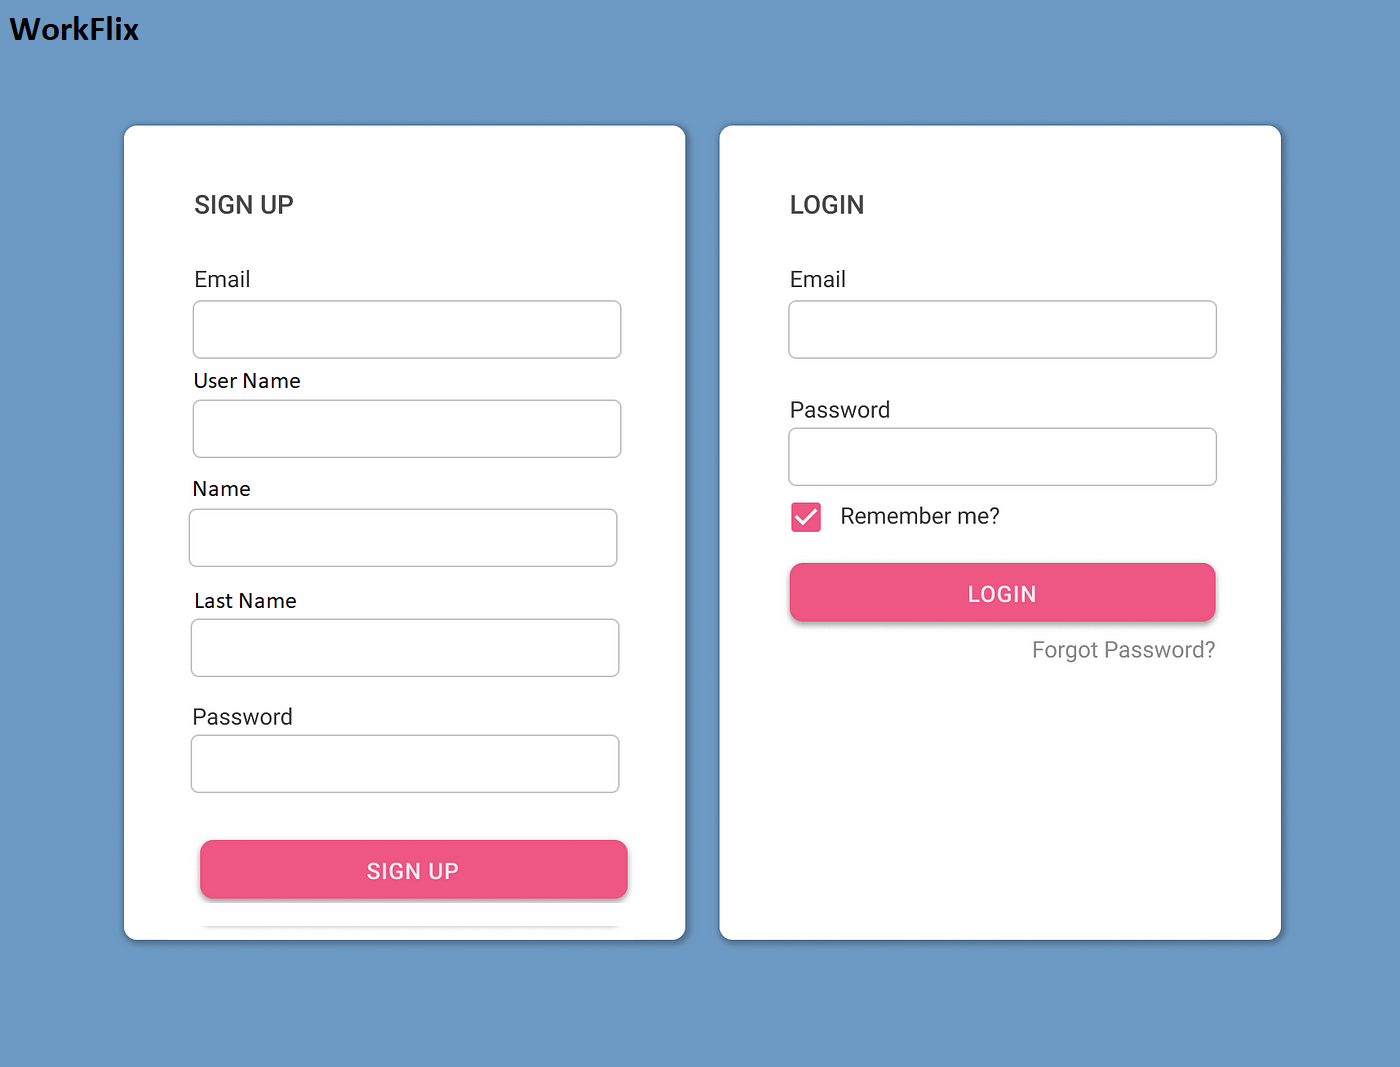
\includegraphics[width=\columnwidth]{images/SignInLogIn.jpg}


\subsection{Analytics}
 Analytics refers to the collection, measurement, and analysis of data related to user behavior and activity within the application.\\
 
 Analytics tools are used to track user interactions with the application, such as page views, clicks, downloads, and other actions that can help developers and business owners understand how users are engaging with the application.\\
 
 Analytics data can also provide insights into user demographics, preferences, and behaviors, which can be used to improve the user experience, optimize marketing campaigns, and make data-driven decisions about the application's development and performance.\\
 
 Popular web analytics tools include Google Analytics, Adobe Analytics, and Mixpanel, among others.

\includegraphics[width=\columnwidth]{images/Analytics.png}
